\documentclass[a4paper, landscape]{article}
\usepackage[margin=0.5cm]{geometry} % Adjust margins as needed
\usepackage{amsmath} % For mathematical symbols and equations
\usepackage{multicol} % For multiple columns
\usepackage{enumitem} % For customizing lists
\usepackage[version=4]{mhchem}
\usepackage{graphicx}
\usepackage{float}
\usepackage{parskip}
\usepackage{vwcol}

\begin{document}
\textbf{\LARGE ENVE422 - Equation Cheat Sheet} \hfill \today
\begin{multicols}{2}
\section*{Introduction}
\subsection*{Quantification}
\begin{figure}[H]
    \centering
    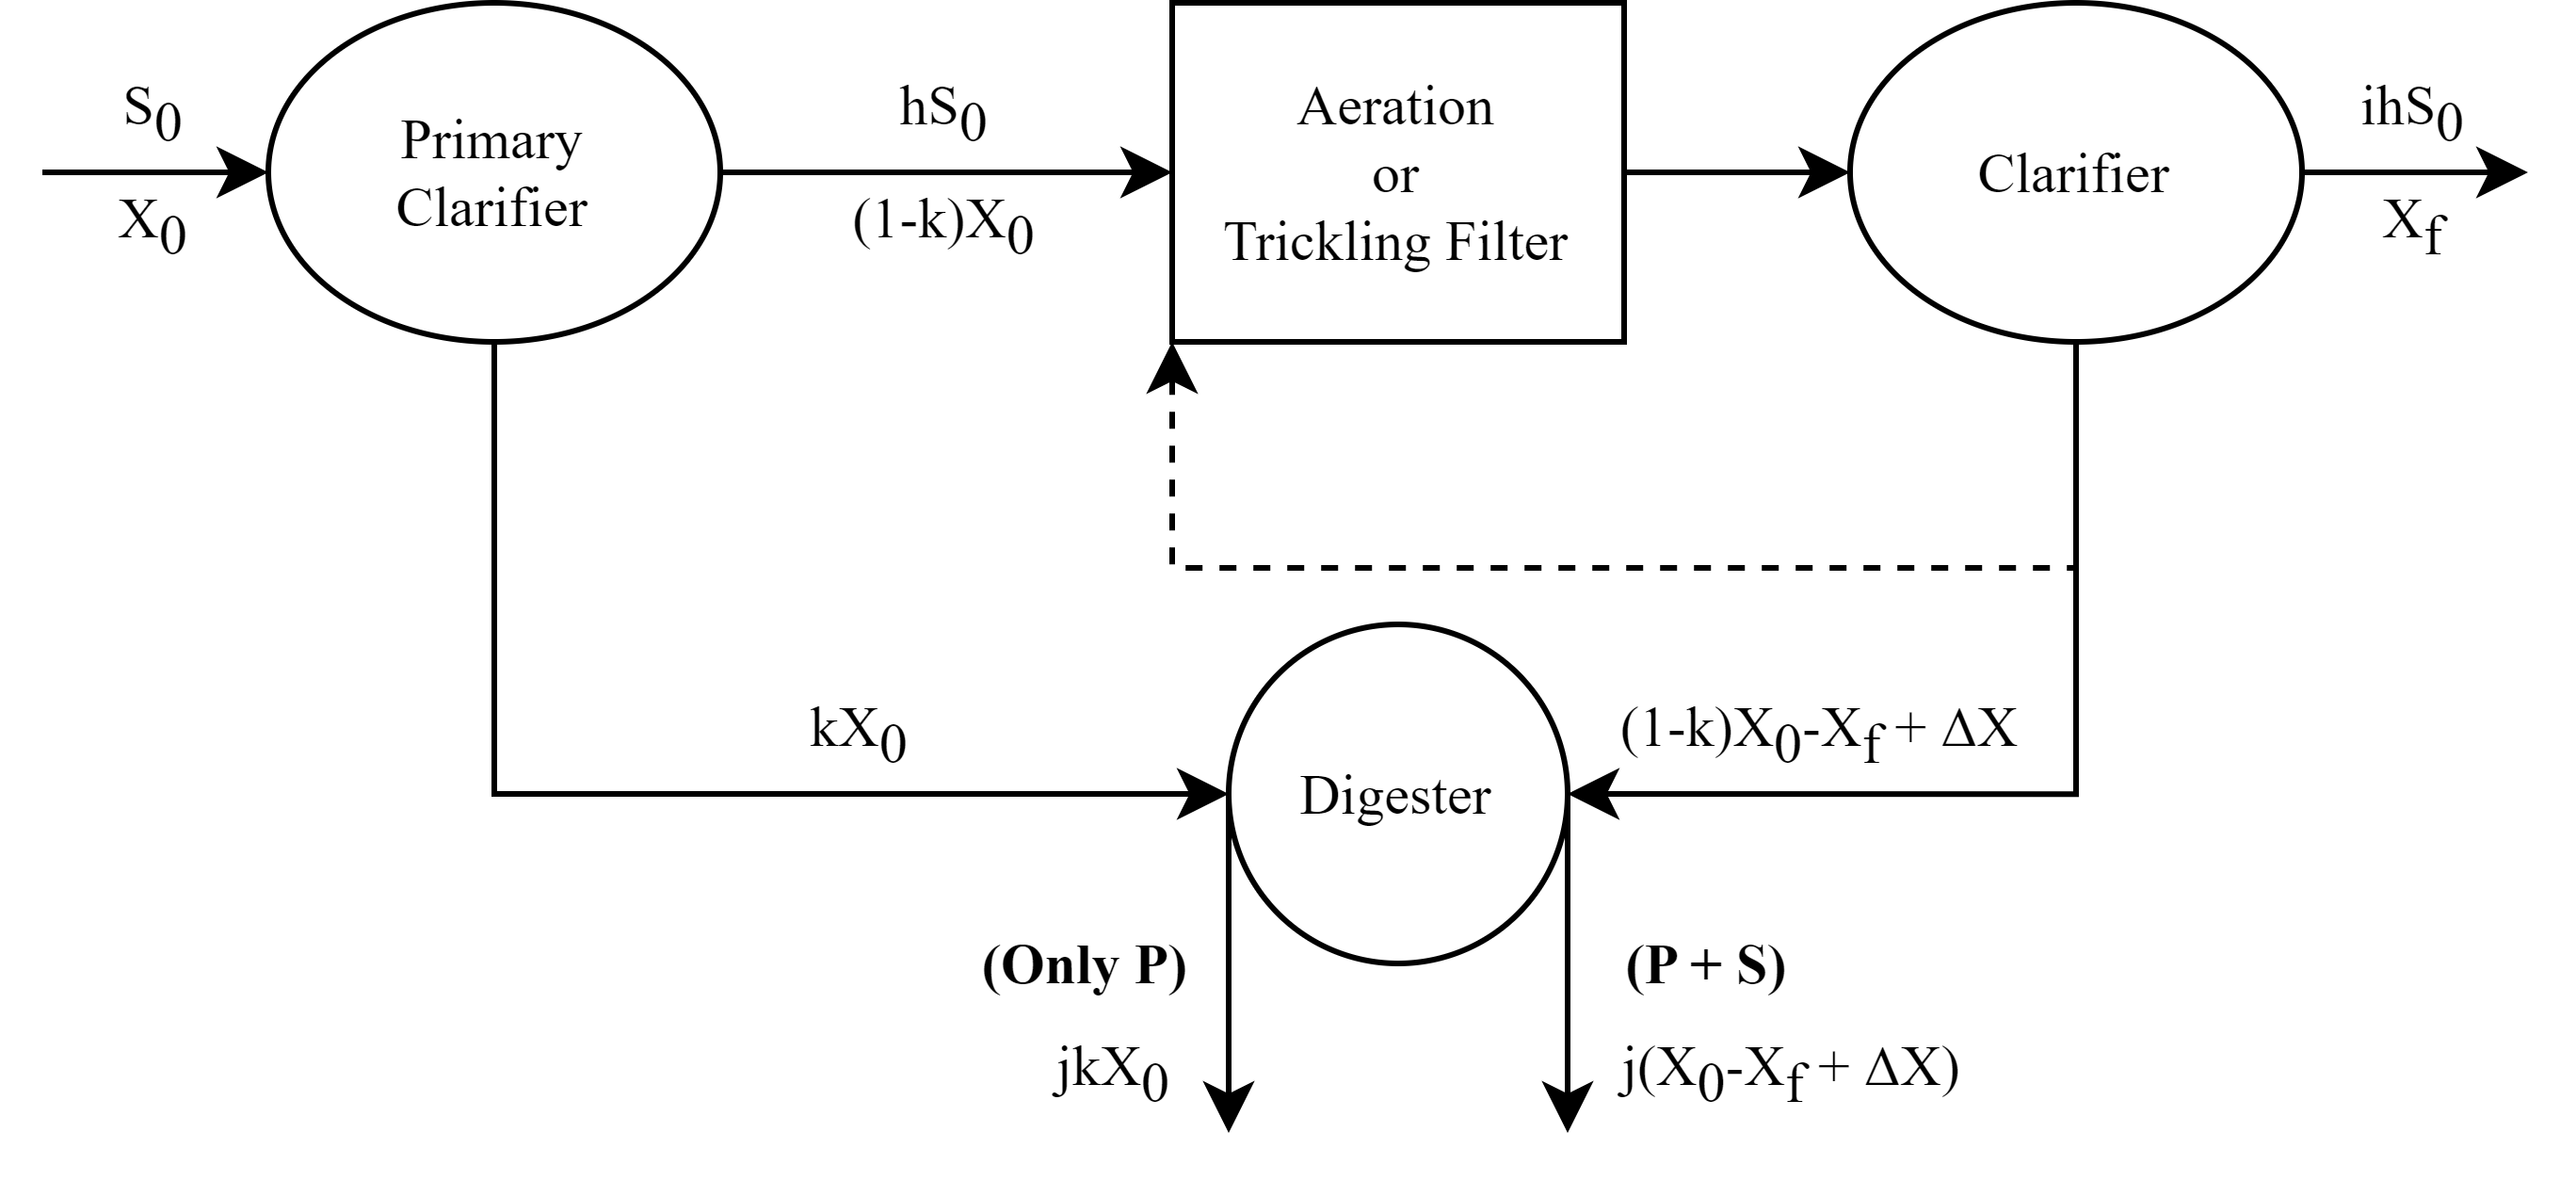
\includegraphics[scale = 1]{SludgeQuantities.png}
    \caption{Flow chart of a sludge generation in a conventional wastewater treatment plant.}
    \label{fig:sludge}
\end{figure}
\columnbreak
\begin{multicols}{2}
\null \vfill
\textbf{\large Parameters}\\
S$_0$ = influent BOD (kg/h)\\
X$_0$ = influent suspended solids (kg/h)\\
h = fraction of BOD not removed in the primary clarifier\\
i = fraction of BOD not removed in the aeration tank\\
X$_f$ = plant effluent suspended solids (kg/h)\\
k = fraction of X$_0$ removed in the primary clarifier\\
j = fraction of solids not destroyed in digester\\
$\Delta$X = net solids produced by biological action (kg/h)\\
Y = Yield = $\Delta$X/$\Delta$S, where:\\
$\Delta$S = hS$_0$ - ihS$_0$
\vfill \null
\columnbreak
\null \vfill
\textbf{\large Typical Values}\\
S$_0$ = 250 * 10$^{-3}$ * Q = kg/h,\\
here 250 mg/L and Q = m$^3$/h\\
X$_0$ = 225 * 10$^{-3}$ * Q = kg/h,\\
here 225 mg/L and Q = m$^3$/h\\
h = 0.7\\
i = 0.1 for well-operated activated sludge\\
i = 0.2 for trickling filters\\
X$_f$ = 20 * 10$^{-3}$ * Q = kg/h,\\
here 20 mg/L and Q = m$^3$/h\\
k = 0.6\\
j = 0.8 (assuming no supernatant withdrawal)\\
Y = 0.5 for activated sludge\\
Y = 0.2 for trickling filters
\vfill \null
\end{multicols}
\end{multicols}
\begin{multicols}{4} % Adjust the number of columns as needed
\subsection*{Definitions}
\textbf{Sludge:} Semi-solid material produced by water and wastewater treatment that needs further treatment for disposal into the environment.
\subsection*{Characteristics}
\textbf{Specific Gravity:} The ratio of the density of a substance to the density of a standard, usually water for a liquid or solid, and air for a gas.
\[
\text{Specific Gravity} = \frac{{\text{density of substance}}}{{\text{density of water}}}
\]
Since there are more than one components in sludges:
\[
\frac{1}{S} = \sum_{i=1}^{n} \frac{W_i}{S_i}
\]
where:\\
S = specific gravity of the sludge,\\
$W_i$ = weight fraction of the $i^{th}$ components of sludge,\\
$S_i$ = specific gravity of the $i^{th}$ component.\\
\textbf{Sludge Volume Index (SVI):} A quick test to settleability of a sludge.
\[
\text{SVI} = \frac{V_{30}*1000}{\text{MLSS}}
\]
where:\\
SVI = Sludge Volume Index (volume occupied by 1 gram of solids, mL/g, but unitless),\\
$V_{30}$ = sludge volume settled in 30 minutes, volume unit,\\
1000 = conversion factor (1000 mg/g),\\
MLSS = Mixed Liquor Suspended Solids, concentration unit.
\subsection*{Rheology}
\textbf{Newtonian fluids:}
\[
\tau = \mu \frac{du}{dy}
\]
where:\\
$\tau$ = shear stress (N/m$^2$ or Pa),\\
$\mu$ = viscosity (Pa·s),\\
$du/dy$ = shear rate (1/s).\\
\textbf{Bingham plastic fluids:}
\[
\tau = \tau_y + \eta \frac{du}{dy}
\]
where:\\
$\tau$ = shear stress (N/m$^2$ or Pa),\\
$\tau_y$ = yield stress (N/m$^2$ or Pa),\\
$\eta$ = plastic viscosity (Pa·s),\\
$du/dy$ = shear rate (1/s).\\
\textbf{Power law model fluids:}
\[
\tau = K \left(\frac{du}{dy}\right)^n
\]
where:\\
$\tau$ = shear stress (N/m$^2$ or Pa),\\
$K$ = fluid consistency index, analogous to viscosity,\\
n = flow behavior index (n < 1 for \textbf{Pseudoplastic fluids} and n > 1 for \textbf{Dilatant fluids}),\\
$du/dy$ = shear rate (1/s).\\
\textbf{Einstein's Equation of Viscosity:}
\[
\mu = \mu_0 (1+2.5\phi)
\]
where:\\
$\mu_0$ = viscosity of suspending medium,\\
$\phi$ = volume fraction of particles.
\subsection*{Dewaterability}
\textbf{Darcy's Law:}
\[
\frac{dV}{d\theta} = \frac{PAK}{\mu L}
\]
where:\\
$dV/d\theta$ = rate of flow, volume per unit time,\\
$P$ = pressure difference,\\
$A$ = area,\\
$\mu$ = viscosity,\\
$K$ = permeability,\\
$L$ = thickness.
For an expression with \textsl{Resistance}:
\[
\frac{dV}{d\theta} = \frac{PA}{\mu LR}
\]
where:\\
$R$ = resistance ($1/K$).\\
\textbf{Considering filter resistance with the cake resistance:}
\begin{equation}
    \frac{dV}{d\theta} = \frac{PA}{\mu (LR+R_f)}
\label{eq:dar1}
\end{equation}
where:\\
$R_f$ = resistance of filter medium.\\
The volume of filter cake can be expressed as:
\[
LA = vV
\]
where:\\
$v$ = volume of cake deposited per unit volume of filtrate ($V$),\\
Substituting L in Equation \ref{eq:dar1}:
\[
\frac{dV}{d\theta} = \frac{PA^2}{\mu (RvV+R_fA)}
\]
It is more convenient to express the cake as dry weight of cake deposited per unit volume of filtrate ($w$). $R$ (resistance by a unit volume) is also changed with $r$ (resistance per unit weight).
\[
\frac{dV}{d\theta} = \frac{PA^2}{\mu (rwV+R_fA)}
\]
where:\\
$w$ = weight of dry cake solids per unit volume of filtrate,\\
$r$ = specific resistance per unit weight.
Assuming constant pressure over time:
\begin{equation}
    \smallint_{0}^{\theta} d\theta = \smallint_{0}^{V} \left( \frac{\mu rwV}{PA^2}+\frac{\mu R_f}{PA}\right)dV \label{eq:dar2}
\end{equation}
Integrating Equation \ref{eq:dar2}:
\begin{equation}
    \frac{\theta}{V} = \frac{\mu rwV}{2 P A^2} + \frac{\mu R_f}{P A} \label{eq:dar3}
\end{equation}
Using Equation \ref{eq:dar3}, experimental data can be obtained by plotting $\theta/V$ and $V$ values on a graph to yield a linear relationship.
\[
y=mx+b
\]
where:\\
$y = \theta/V$\\
$m = \text{ slope } = \mu rw / 2 PA^2$\\
$x = V$\\
$b = \text{ intercept } = \mu R_f / PA$
$r$ can be obtained by using slope.\\
For $w$, if the filtrate SS can be assumed negligible (which is reasonable), i.e., CF = 0, then:
\[
w = \frac{C_KC_0}{(C_K-C_0)}
\]
If in \%:
\[
w = \frac{C_KC_0}{100(C_K-C_0)}
\]
where:\\
$C_K$ = cake solids concentration (\%),\\
$C_0$ = feed solids concentration (\%).\\
\textbf{Capillary Suction Time:}
\[
\chi = (D_2^2 - D_1^2)\left(\frac{\pi d}{ A P }\right)\left(\frac{\mu C}{t}\right)
\]
where:\\
$D_1$ = 1$^{st}$ sensor location (diameter),\\
$D_2$ = 2$^{nd}$ sensor location (diameter),\\
$d$ = filter paper depth (thickness),\\
$A$ = area of the bottom of the collar, sludge area,\\
$P$ = capillary suction, analogous to head term in Darcy's equation,\\
$\mu$ = filtrate viscosity,\\
$C$ = sludge solids concentration,\\
$\chi$ = sludge filterability incorporating permeability,\\
t = capillary suction time (CST).
\section*{Stabilization}
\textbf{Modified Buswell Equation:}
\begin{multline}
    \ce{C_aH_bO_cN_d + $\left(\frac{4a - b - 2c + 3d}{4}\right)$H2O\\ -> $\left(\frac{4a + b - 2c - 3d}{8}\right)$CH4 \\+ $\left(\frac{4a - b + 2c + 3d}{8}\right)$CO2 + $d$NH3}
    \label{eq:Buswell}
\end{multline}
Equation \ref{eq:Buswell} is used for the determination of \textbf{anaerobic decomposition} of an organic material.
\end{multicols}
\end{document}
